\documentclass[fleqn]{jbook}
\usepackage{physpub}

\begin{document}

\begin{question}{専攻 問題3}{}


磁場$H$中での大きさ$J\;(=1/2,1,3/2,\cdots)$のスピンのエネルギー
固有値$\varepsilon_m$は、
%
\[ \varepsilon_m = g\mu_BHm, \hspace{10mm}(m=-J,-J+1,\cdots,J-1,J) \]
%
で与えられる。ここで、$m$は磁気量子数、$g$は$g$因子、$\mu_B$はボーア
磁子である。このようなスピンを単位体積中に$n$個含み、温度$T$の熱平衡
状態にある系について、以下の問に答えよ。ただし、ボルツマン定数を$k$
とし、スピンの間の相互作用は考えない。


\begin{subquestions}
\SubQuestion
  この系の単位体積あたりの分配関数は次式で与えられることを示せ。
%
  \[ Z = \left(\frac{\sinh[(2J+1)x/2J]}{\sinh(x/2J)}\right)^n,%
     \hspace{1cm}x=\frac{g\mu_BJH}{kT} \]
%

\SubQuestion
  この系の単位体積あたりの比熱$C$を次式で定義されるブリルアン関数
  $B_J(x)$の導関数を用いて表せ。
%
  \[ B_J(x) = \frac{2J+1}{2J}\coth\left(\frac{2J+1}{2J}x\right)
             -\frac{1}{2J}\coth\left(\frac{x}{2J}\right) \]
%

\SubQuestion
  温度が(a)高い場合($x\ll 1)$と(b)低い場合($x\gg J)$について、
  比熱$C$の近似形を求めよ。


\SubQuestion
  前問の結果に基づき、$J=1/2$に対して、比熱$C$の温度依存性の概略を
  図示し、このような温度依存性となる物理的理由を述べよ。なお、図は
  縦軸を$C/nk$、横軸を$kT/g\mu_BJH$とせよ。


\SubQuestion
  古典スピンの極限(積$g\mu_BJ$が一定のまま
  $J\rightarrow \infty,\;g\mu_B\rightarrow 0$とした場合)
  における比熱$C$を求めよ。さらに、その温度依存性の概略を示せ。
  なお、図は前問同様、縦軸を$C/nk$、横軸を$kT/g\mu_BJH$とせよ。

--------------------------------------------------------------------------------------------------------------\\
(参考)ブリルアン関数
%


\begin{minipage}{90mm}
  右図に$J=1/2,1,2,4,8$に対するブリルアン関数を示す。\\
  近似式(証明なしに用いてよい)
  \begin{eqnarray*}
    B_J(x) &\approx& \left\{\begin{array}{ll}%
      \ds \frac{J+1}{3J}x &%
      (x\ll 1) \\[2mm]
      \ds 1-\frac{1}{J}\exp\left(-\frac{x}{J}\right) &%
      (x\gg J)%
    \end{array}\right.\\
%
    \coth(x) &\approx& \left\{\begin{array}{ll}%
      \ds \frac{1}{x}+\frac{x}{3}\quad\quad\quad\quad\;\;&
      (x\ll 1)\\[2mm]
      \ds 1+2e^{-2x} &
      (x\gg 1)%
    \end{array}\right.
  \end{eqnarray*}
\end{minipage}
\begin{minipage}{70mm}
  \begin{center}
    \mbox{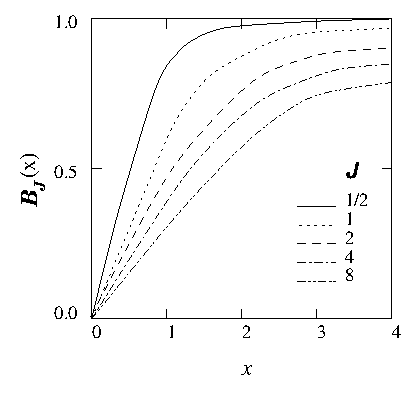
\includegraphics[clip]{1994phy3-1.eps}}
  \end{center}
\end{minipage}


\end{subquestions}
\end{question}
\begin{answer}{専攻 問題3}{}

\begin{subanswers}
\SubAnswer
  各スピン間の相互作用は考えないので、全系の分配関数は1つのスピンの
  の分配関数の $n$ 乗である。
%
  \begin{eqnarray*}
    Z &=&   \left( \sum_{m=-J}^{J} \exp\left(%
            \frac{g\mu_B H}{kT}m\right) \right)^{n}%
       =    \left( \sum_{m=-J}^{J} \exp\left(%
            \frac{x}{J}m\right) \right)^{n}%
       =  \left( \frac{e^{-Jx/J}(e^{(2J+1)x/J}-1)}%
                 {e^{x/J}-1} \right)^{n} \\
      &=&  \left( \frac{e^{(2J+1)x/2J}-e^{-(2J+1)x/2J})}%
                 {e^{x/2J}-e^{-x/2J}} \right)^{n}%
       =   \left( \frac{\sinh[(2J+1)x/2J]}{\sinh(x/2J)}\right)^{n}
  \end{eqnarray*}



\SubAnswer
  平均エネルギー$U$は
%
  \begin{eqnarray*}
    U &=& \frac{\sum{\varepsilon e^{-\beta \varepsilon}}}%
          {\sum e^{-\beta \varepsilon}}%
       = - \Partial{}{\beta} \ln{Z}%
       = -ng \mu_B JH\Partial{}{x} \left(%
            \ln{(\sinh{(2J+1)x/2J})}-\ln{(\sinh{x/2J})} \right) \\
      &=& -ng \mu_B JH \left(%
           \frac{2J+1}{2J}\coth{\frac{2J+1}{2J}x}%
          -\frac{1}{2J}\coth{\frac{1}{2J}x} \right)%
       =  -ng \mu_B JH B_J(x) \\[2mm]
    \Yueni C &=& \Deriver{U}{T}%
       =  \Deriver{x}{T} \Deriver{U}{x}%
       =  \frac{n(g \mu_B JH)^2}{kT^2}B_J'(x)
       =  nkx^2 B_J'(x)
  \end{eqnarray*}


\SubAnswer
  \[ T \rightarrow \makebox[10mm]{\bf\rm large},\quad x \ll 1 \qquad%
     C \simeq nkx^2 \frac{J+1}{3J}%
       =      \frac{J+1}{3J} nkx^2 \]
  \[ T \rightarrow \makebox[10mm]{\bf\rm small},\quad x \gg J \qquad%
     C \simeq \frac{nkx^2}{J^2}\exp{\left(-\frac{x}{J}\right)} \]
%

\SubAnswer
  \parbox[t]{88mm}{
  $J=1/2$ なので
%
  \[ x\ll 1 \qquad \frac{C}{nk} \simeq x^2  \]
  \[ x\gg J \qquad \frac{C}{nk} \simeq 4x^2 \exp(-2x) \]
%
  $T \rightarrow$大では、スピンの向きは全くランダムとなり、\\
  $\Mean{E} \rightarrow 0$、よって $C \rightarrow 0$。\\
  $T \rightarrow$小では、エネルギーを最小にするため、スピンがすべて
  $m=+J$にそろってしまうので $C \rightarrow 0$。
  }\parbox[t]{75mm}{\vspace*{-5mm}
  \begin{center}
    \mbox{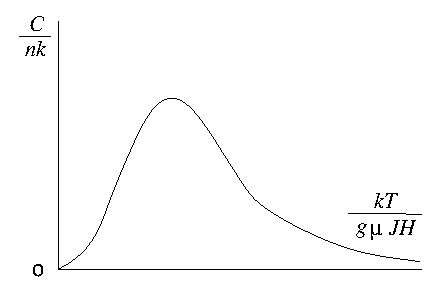
\includegraphics[clip]{1994phy3-2.eps}}
  \end{center}}


\SubAnswer
  $x,\,g \mu_B J$を有限の一定値にしたまま、$J \rightarrow \infty$とする。
%
\begin{align*}
	\lim_{J\rightarrow\infty}B_J(x)
	& = \lim_{J\rightarrow\infty}
		\biggl(\frac{2J+1}{2J}\coth\frac{2J+1}{2J}x
			-\frac{1}{2J}\coth\frac{1}{2J}x\biggr) \\
	& =  \coth x
		-\lim_{J\rightarrow\infty}\frac{1}{2J}
			\biggl(\frac{2J}{x}+\frac{1}{3}\frac{x}{2J}\biggr) \\
	& =  \coth x-\frac{1}{x}
\end{align*}
  \[ \lim_{J\to\infty} U%
      = -ng \mu_B JH \lim_{J\to\infty}%
         \left( \frac{2J+1}{2J}\coth{\frac{2J+1}{2J}x}%
              - \frac{1}{2J}\coth{\frac{1}{2J}x} \right)%
      =  -ng \mu_B JH \left( \coth x -\frac{1}{x} \right) \]
%
従って、比熱は
\begin{align*}
	C & = nkx^2\Deriver{}{x}\biggl(\coth x-\frac{1}{x}\biggr) \\
	& = nk(1-x^2\cosech^2x)
\end{align*}
となる。よって、


  \parbox[t]{88mm}{
  \begin{eqnarray*}
     \hspace{-10mm}x\ll 1 \qquad%
     U &=& -ng \mu_B JH \left( \frac{x}{3} \right) \\
     \Yueni%
     C &=& \Deriver{U}{T} =\frac{n(g\mu_BJH)^2}{3kT^2}%
        = \frac{nkx^2}{3} \\
     \hspace{-10mm}x\gg 1 \qquad%
     U &=& -ng \mu_B JH \left( 1+2e^{-2x}-\frac{1}{x} \right) \\
     \Yueni%
     C &=& \Deriver{U}{T}%
       = \frac{n(g\mu_BJH)^2}{kT^2}\left(\frac{1}{x^2}-4e^{-2x}\right)\\
       &=& nk(1-4x^2e^{-2x})
  \end{eqnarray*}
%
  }\parbox[t]{75mm}{
  \begin{center}
    \mbox{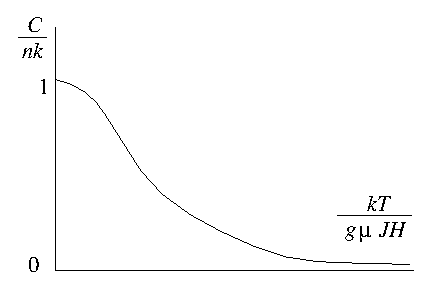
\includegraphics[clip]{1994phy3-3.eps}}
  \end{center}}

\end{subanswers}
\end{answer}


\end{document}
